%!TEX root = ../../super_main.tex
\section{Structural Sensor Data}
\label{sec:structural_sensor_data}
Because a continuous output from all sensors is not viable option when gathering information, we want to give the customers the ability to configure what and when the outputs should be measured. This should be done in such a way that the customers can specify what data is important to them and still avoid draining the resources of the participants devices. For this reason we have designed a way to provide customers with the possibility to configure the temporality of the data that they want. 
\\\\
We see all the different sensors as something we can eaves drop in at all times meaning that we can retrieve a measurement from any sensor at all times. For a better understanding of the structure that have been designed for the measurement we invite the reader to look at \figref{fig:sample_temporality} while reading the following description of the concept. A single measurement from the continuous sensors does not make sense on their own, for instance a single measurement from accelerometer does describe the context in which the participants exist. However if we get a stream of accelerometer measurements, we would be able to describe the motion of the device. For this reason we introduce a concept called \emph{sample}, where we gather measurements with intervals to cover these continuous sensor outputs. On the other hand, we also have some sensors that does not add much information to measure in as great granularity. The location of the participant (through GPS) is a sensor that does not change often, and is unlikely to have great differences in values. By making it possible to measure these two types of sensors differently, one would be able to determine if the user is driving a car (the accelerometer is not changing much but the location changes) or is biking (the a accelerometer is fluctuating and the location is still changing, but not at much). If a customer wanted to measure this particular pattern they would specify that the sample of a location should have a measurement frequency that is longer than the accelerometer.
\todo[inline]{Rikke: Explain the figure better, it is only explained through an example}
\begin{figure}[!htbp]
    \centering
    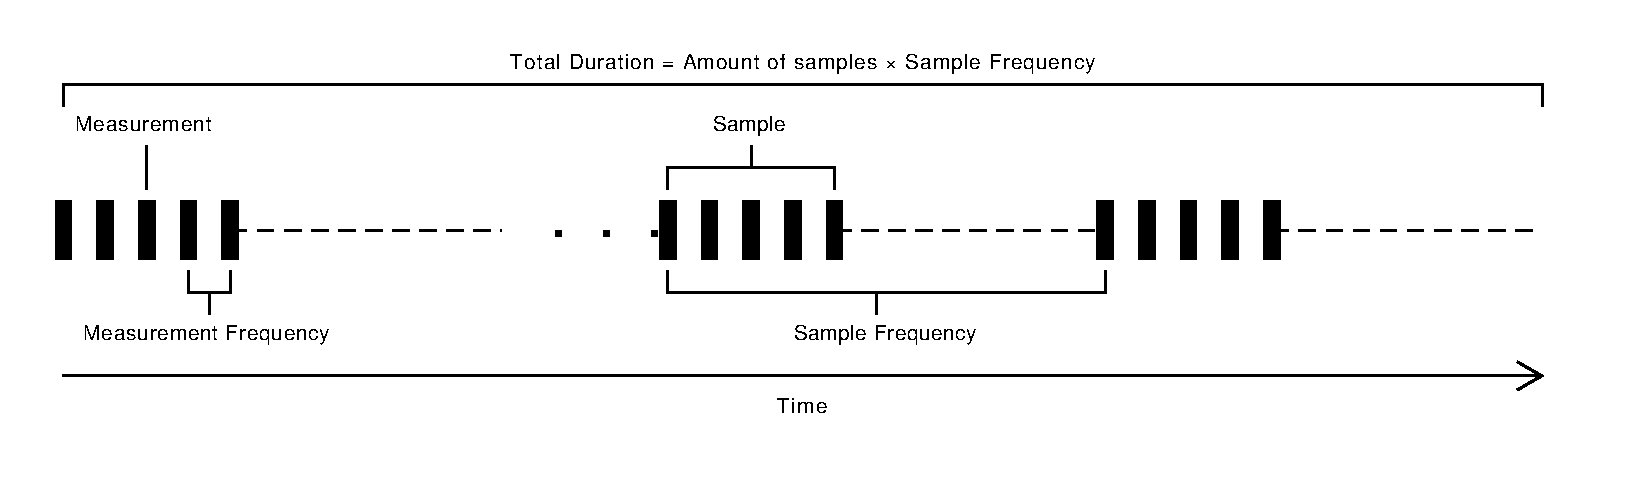
\includegraphics[width=\textwidth]{gathering_sensor_data/sample_temporality.pdf}
    \caption{Overview of sample and measurement temporality.}
    \label{fig:sample_temporality}
\end{figure}
\FloatBarrier

Furthermore, we want the customer to configure how often these samples should be gathered, and for that reason we allow them to define a sample frequency. And lastly the customer is also able to define the total duration of the gathering data.

\todo[inline]{Vi har reelt 3 forskellige tider: Hvor længe skal et sample vare, hvor ofte skal vi tage et sample, hvor længe skal der gå imellem measurements i et sample? På grund af at sensore i Android giver svar når de har lyst, er det ikke sikkert at der kommer den samme mængde measurements i hver sample. Vi skal overveje om det giver mening, eller om det er vigtigere for kunden at hvert sample med garenti indeholder x measures. Problemet med dette er så at vi ikke kan sætte nogen garenti for hvornår disse measures reelt kommer.}